% =====================================================================
%  What Undecidability Feels Like From the Inside
%  ALife submission — DRAFT
%
%  Built from holes/tech-notes/TN-propagator-paper.md (2026-07-16).
%  Structure follows that note's core decision: ONE paper, Paper B's
%  thesis, with Paper A as the first half.
%
%  VENUE: Artificial Life (MIT Press), category ARTICLE.
%    "A manuscript reporting original research, typically of 6,000 to
%     12,000 words."  Other categories: Letters <=2000, Fast Track ~2000,
%     Reports <=2000, Reviews >=12000.
%    The journal requires APA-7 citations, which is why we are on apa7 and
%    why the biblatex line below is `style=apa` -- that matches the
%    journal's own template verbatim, so refs.bib and every \parencite
%    port across unchanged if we later swap the class.
%    Submission: https://mc.manuscriptcentral.com/artificiallife (PDF)
%    Guidelines: https://direct.mit.edu/artl/pages/submission-guidelines
%
%  BODY WORD COUNT (measured, draft apparatus hidden): ~3,540.
%    ~2,460 words UNDER the Article floor. The two unwritten sections
%    (Background, Discussion) are roughly that size. See README.md.
%
%  Class option `man` = APA-7 manuscript (double-spaced, figures at end
%  unless floatsintext). Switch `man` -> `jou` for the two-column
%  journal look. `doc` for a plain single-space read-through.
%
%  Build:  latexmk -pdf main.tex     (biber is wired via latexmkrc)
% =====================================================================
\documentclass[man,12pt,floatsintext]{apa7}

\usepackage[american]{babel}
\usepackage{csquotes}
\usepackage{amsmath,amssymb}
\usepackage{booktabs}
\usepackage{graphicx}
\usepackage{xcolor}
\usepackage[style=apa,backend=biber]{biblatex}
\addbibresource{refs.bib}

% ---- draft apparatus -------------------------------------------------
% \draftnotestrue -> show; \draftnotesfalse -> hide for a clean read.
\newif\ifdraftnotes
\draftnotestrue

\definecolor{owedcol}{HTML}{B03A2E}
\definecolor{notecol}{HTML}{1F618D}

% An OWED item: something a reviewer will ask for that we do not yet have.
\newcommand{\owed}[1]{\ifdraftnotes\textcolor{owedcol}{\small\textbf{[OWED:} #1\textbf{]}}\fi}
% A drafting note to ourselves.
\newcommand{\dnote}[1]{\ifdraftnotes\textcolor{notecol}{\small\textbf{[NOTE:} #1\textbf{]}}\fi}

% ---- notation --------------------------------------------------------
\newcommand{\sig}{\sigma}
\newcommand{\bit}[1]{\mathrm{bit}[#1]}

\title{What Undecidability Feels Like From the Inside: A Rule-Space
Propagator and the Limits of Edge-of-Chaos Measurement}

\shorttitle{Limits of Edge-of-Chaos Measurement}

\author{Joseph Corneli}
\affiliation{Hyperreal Enterprises}

\authornote{\addORCIDlink{Joseph Corneli}{0000-0003-1330-4698}

\dnote{ORCID copied from prior work --- confirm. Co-authorship of the
original 2015 experiment (Ewen Maclean) may warrant an invitation; that is
Joe's call, not the draft's.}

Correspondence concerning this article should be addressed to Joseph
Corneli. E-mail: holtzermann17@gmail.com}

\abstract{%
A single off-by-one error, written in Emacs Lisp in 2014 and undisturbed
for twelve years, converts mutation in a meta-cellular automaton from a
random walk over rule space into a \emph{constraint propagator} over the
rule's bit-planes. We reconstruct the effect from the original code,
correct two claims in the paper that first published it, and generalise
it to a family indexed by permutations $\sig$ of the eight truth-table
positions, a sampled majority of which (112/202) sustain non-trivial
dynamics. We then prove the family's central question
unanswerable in the terms it invites: a live operator and a dead one are
\emph{exactly conjugate} as isolated stochastic systems, so no property
of $\sig$ alone separates them. The second half reports our attempt to
locate these systems relative to the edge of chaos. Every
instrument failed, and failed informatively --- most sharply as a
\emph{pincer}: a phenotype transport statistic with a positive anchor but
no null, and a genotype counterpart with nulls but no anchor. This is not
a catalogue of engineering mistakes.
Wolfram class membership and nilpotency are undecidable, and Rule 110's
universality was established by construction, never by measurement;
``build an edge-of-chaos instrument'' is not well-posed. Across three
metrics with matched controls (Euclidean, Fisher--Rao, Wasserstein-1),
the 20{,}256 propagator orbits form a continuum with no \emph{metric}
joints --- and yet the family partitions exactly, by an algebraic
invariant no distance can see. A Boolean fixed point exists iff every
cycle of the shape map is even; all-even operators, $(7!!)^2 = 11{,}025$
of $40{,}320$ by a closed form the census confirms, die five times as
often as the rest. Two permutations one transposition apart fall on
opposite sides, so our fail bank is a fail bank of \emph{distances}.
We offer it as the contribution, with two surviving methods: a certified mean-field
bound making 205M transport distances tractable, and Ollivier--Ricci
curvature as navigation for a space with no metric clusters.}

\keywords{cellular automata, edge of chaos, undecidability, reproducibility,
optimal transport, information geometry, negative results}

\begin{document}
\maketitle

% =====================================================================
\section{Introduction}
% =====================================================================

\dnote{Intro is the least-settled prose in the draft. It currently states
the thesis and the route. It does not yet \emph{sell} --- the ALife framing
(Langton's $\lambda$ as this community's long-running quarry) should
probably arrive in the first paragraph rather than the third.}

This paper has two halves and one thesis. The first half is about an
object: a constraint propagator over the bit-planes of a cellular
automaton rule, which we found by reconstructing a figure from a 2015
paper \parencite{corneli2015search} and discovering that the figure was
produced by a bug. The second half is about a failure: we could not
measure where that object sits relative to the edge of chaos, and neither,
we will argue, could anyone else, because the thing we were trying to
measure is undecidable.

The two halves are not independent. The propagator family is an unusually
clean setting in which to ask the edge-of-chaos question --- it is finite
($8! = 40{,}320$ operators), exhaustively enumerable, and equipped with an
exact algebraic structure. If the question were going to be answerable
anywhere, it would be answerable here. It is not answerable here. That is
worth more than another proxy.

The edge of chaos has been this community's quarry since
\textcite{langton1990computation} proposed $\lambda$ and
\textcite{packard1988adaptation} evolved automata toward it. It has also
been this community's most durable source of negative results, of which
\textcite{mitchell1993revisiting} remains the sharpest: the evolved
automata were not, on inspection, doing what the edge-of-chaos story said
they were doing. We place ourselves in that lineage and try to say
something it did not: that the failure has a proof behind it.

\subsection{Contributions}

\begin{enumerate}
  \item \textbf{The propagator} (Section~\ref{sec:propagator}). We
  reconstruct Figure~8 of \textcite{corneli2015search} from the original
  2014 Emacs Lisp, and correct that paper's own account of it in two
  places, using its own published artefact as evidence.

  \item \textbf{The conjugacy theorem} (Section~\ref{sec:conjugacy}). A
  live operator and a dead operator are exactly conjugate as isolated
  stochastic systems (2048/2048 transitions commute). Therefore no
  $\sig$-only property separates live from dead. This forecloses an
  entire class of explanation, including one we had ourselves fitted to
  12/12 cases.

  \item \textbf{An exhaustive census} (Section~\ref{sec:census}) of all
  20{,}256 mirror orbits covering all 40{,}320 operators, fingerprinted
  and reproducible, plus exact fixed points for every operator computed
  as a $256 \times 256$ Markov chain rather than sampled.

  \item \textbf{The fail bank} (Section~\ref{sec:failbank}), which we
  regard as the paper's centre of gravity, and in particular
  \emph{the pincer}: two transport statistics of which each has exactly
  what the other lacks.

  \item \textbf{The undecidability argument} (Section~\ref{sec:theorem}):
  why the fail bank is a theorem's shadow and not a to-do list.

  \item \textbf{Two methods that survived} (Section~\ref{sec:methods}): a
  certified mean-field lower bound on Wasserstein-1, and Ollivier--Ricci
  curvature as a navigation primitive for a joint-free space.
\end{enumerate}

% =====================================================================
\section{Background}
% =====================================================================

\owed{This section is a stub. TN ``Known weaknesses'' item 4 records
related-work grounding as a literature search that has not been run.
\texttt{refs.bib} has the named ancestors --- Langton, Packard,
Mitchell/Crutchfield/Hraber, Culik \& Yu, Kari, Cook, {\v C}encov,
Ollivier --- but nobody has read them \emph{for this paper} and positioned
against them. Do not submit with this section in its present state.}

\subsection{The edge of chaos and its negative results}

\dnote{Wanted here: $\lambda$ \parencite{langton1990computation}; Packard's
evolution toward the critical regime; and
\textcite{mitchell1993revisiting} as our closest ancestor --- they found
the evolved automata were exploiting something other than criticality, we
find the measurement itself is not well-posed. Their negative is
empirical; ours has \textcite{culik1988undecidability} behind it. That
contrast is the paper's position in the literature and should be stated
explicitly.}

\subsection{Meta-cellular automata}

\dnote{Wanted: the MetaCA setting from \textcite{corneli2015search} ---
each cell carries a \emph{rule byte} (genotype) as well as a state
(phenotype), and rules evolve by mutation and blending with neighbours.
Needs a compact formal statement; currently the reader meets it for the
first time in Section~\ref{sec:reconstruction}, which is too late.}

% =====================================================================
\section{The Propagator}
\label{sec:propagator}
% =====================================================================

\subsection{Reconstructing Figure 8}
\label{sec:reconstruction}

Figure~8 of \textcite{corneli2015search} shows a MetaCA genotype settling
into an attractor of two rules differing in a single bit. We reproduced it
from the original code at commit \texttt{2f62f59}
(Figure~\ref{fig:figure8}), and in doing so found why it happens.

The mutation operator \texttt{mutate-genotype-n} draws a zero-based
position \texttt{pos} and then writes at \texttt{(goto-char pos)}. Emacs
buffers are one-based, and \texttt{(goto-char 0)} does not error --- it
silently clamps to \texttt{point-min}. The intended random walk over the
eight truth-table bits is therefore not what runs. What runs couples the
bit-planes: source position 0 and source position 1 both write bit~0,
positions $2..7$ write bits $1..6$, and bit~7 is never written at all.

\begin{figure}[htbp]
  \centering
  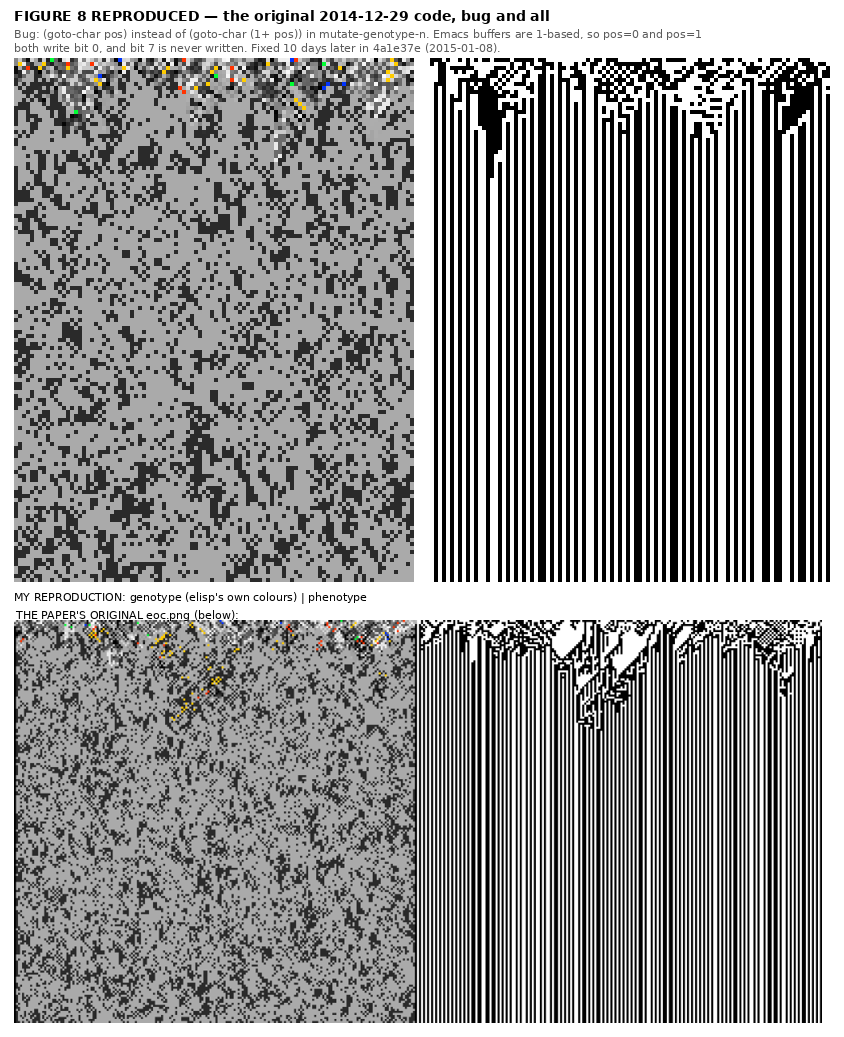
\includegraphics[width=0.62\linewidth]{figures/figure8_REPRODUCED.png}
  \caption{Figure~8 of \textcite{corneli2015search}, reproduced from the
  original 2014 Emacs Lisp at \texttt{2f62f59}. The genotype settles to an
  attractor on two rules differing in one bit. The published text names
  these as rules 0 and 128; they are in fact 42 and 170 (see
  Section~\ref{sec:corrections}).}
  \label{fig:figure8}
\end{figure}

\subsubsection{Two corrections to the published account}
\label{sec:corrections}

\paragraph{The attractor is 42/170, not 0/128.}
The 2015 text states that the genotype flutters between rules 0 and 128.
It does not; it flutters between 42 and 170. The proof comes from the
paper's own artefact. Rule 0 renders as \texttt{\#000000} and rule 128 as
\texttt{\#808080} under the \texttt{256ca.el} colour assignment, and
neither colour appears anywhere in the published \texttt{eoc.png}. That
image's dominant colours are \texttt{\#2a2a2a} (126k px) and
\texttt{\#aaaaaa} (36k px) --- exactly the colours \texttt{256ca.el}
assigns to rules 42 and 170. The structural description in the original
paper (two rules differing in one bit) was correct; the identities were
not.

\paragraph{``Only ever flips the first bit'' is a gloss.}
The published prose describes the bug as only ever flipping the first bit.
Instrumenting the writes directly --- observing \texttt{goto-char}
\emph{after} Emacs clamps, so that the histogram measures writes rather
than inferring them from source --- gives a different and more interesting
picture. Over 87{,}632 measured writes
(Table~\ref{tab:writes}), bit~0 takes 24.946\%, which is the predicted
$2/8$; bits $1..6$ take approximately 12.5\% each; and bit~7 takes
0.000\%. The operator \emph{doubles} bit~0 and \emph{never} writes bit~7.
An independent 216{,}000-write control under the blending-mutation arm
gives the same shape (bit~0 at 24.912\%), and the repaired 2015
implementation is uniform across all eight positions.

\begin{table}[htbp]
  \centering
  \caption{Measured write positions under the 2014 Baldwin arm
  (87{,}632 writes). Positions are zero-based written bits, observed after
  Emacs clamps \texttt{goto-char}.}
  \label{tab:writes}
  \begin{tabular}{lrrrrrrrr}
    \toprule
    written bit & 0 & 1 & 2 & 3 & 4 & 5 & 6 & 7 \\
    \midrule
    count & 21{,}861 & 11{,}062 & 10{,}932 & 10{,}976 & 10{,}906 & 10{,}942 & 10{,}953 & 0 \\
    share (\%) & 24.946 & 12.623 & 12.475 & 12.525 & 12.445 & 12.486 & 12.499 & 0.000 \\
    \bottomrule
  \end{tabular}
\end{table}

\subsubsection{A control the reconstruction needed}

The Figure-8 commit's own default evolution function is a Baldwin variant
\parencite{baldwin1896new,hinton1987learning}, not the blending-mutation
function our reconstruction used. Because the alias is misleading, we ran
the control. The 2014 Baldwin default reaches the exact 42/170 attractor
in \textbf{0/15} seeds; blending-mutation reaches it in \textbf{15/15}
(Figure~\ref{fig:x15}). The reconstruction used the right function despite
the alias --- and the published figure is \emph{not} robust to the
default-function choice, which is precisely why the control was necessary.
We report this as an honest negative about the original: the picture
reproduces, but not under the function the file defaults to.

\begin{figure}[htbp]
  \centering
  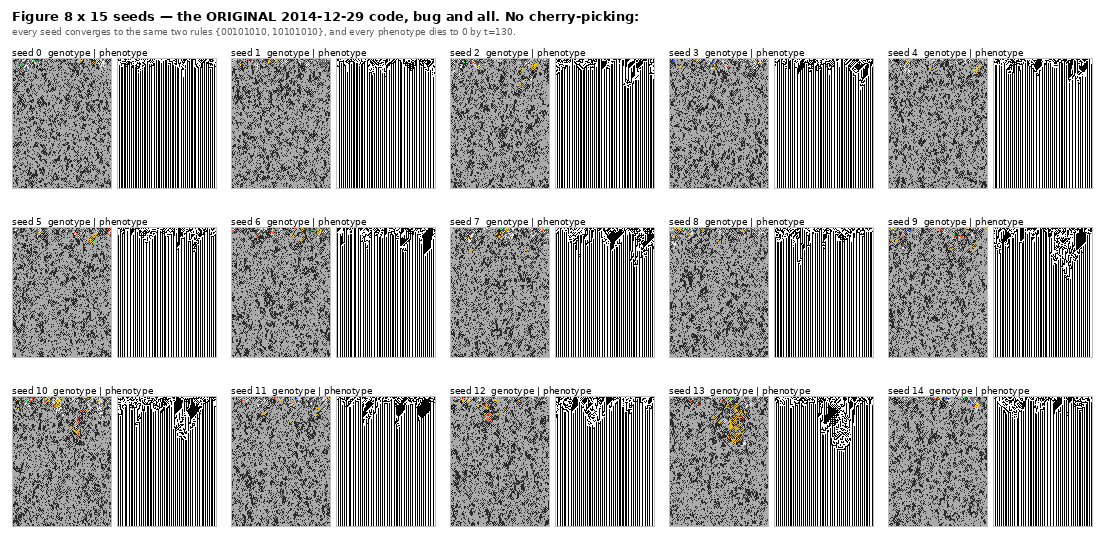
\includegraphics[width=\linewidth]{figures/figure8_x15_repro.png}
  \caption{Fifteen seeds under blending-mutation, no cherry-picking. All
  fifteen reach the exact $\{42,170\}$ attractor. The 2014 Baldwin default
  reaches it in none of fifteen.}
  \label{fig:x15}
\end{figure}

\subsection{Baldwin is a composition of propagators}
\label{sec:baldwin-composition}

The control of Section~\ref{sec:propagator} treated the 2014 Baldwin default as
an obstacle: a misleading alias that had to be ruled out before the
reconstruction could stand. Read a second time it is the more interesting
object, because it is not a primitive at all.

Stripped of Elisp, \texttt{evolve-sigil-with-blending-baldwin} counts how many of
the three old context values equal the new state and then mutates
\texttt{(1- mutations)} times. Zero matches requests $-1$ steps, and
\texttt{(dotimes (j -1) ...)} runs zero times. So the rule is
\begin{quote}
  \emph{context already matches what just happened} $\rightarrow$ mutate;\quad
  \emph{context differs} $\rightarrow$ hold.
\end{quote}
That is $\mathrm{switch}(\textit{local-condition}, \textit{propagator},
\textit{no-op})$: a composition whose constituents are a propagator and the
identity, selected by a locally-readable sign. The 2014 file wrote an
\emph{endogenous} objective --- it needs no edge-of-chaos oracle because it never
asks the question. It reads its own boredom.

\subsubsection{What the composition buys}

Not a new attractor. Baldwin reaches the diagnostic $\{42,170\}$ attractor in
$0/15$ seeds (Section~\ref{sec:propagator}); its constituents do not compose to a
new fixed point. What it buys is a \emph{rate}. Instrumented over 15 seeds of
unedited vendored Elisp (104{,}400 interior calls), the requested-mutation
histogram is $-1$: 1{,}869 ($1.79\%$); $0$: 22{,}539 ($21.59\%$); $1$: 72{,}352
($69.30\%$); $2$: 7{,}640 ($7.32\%$). So $76.62\%$ of interior calls request a
positive mutation, at $0.8114$ steps per cell. The contrast is the point:
\texttt{blending-mutation} requests mutation on $100\%$ of cells at a fixed two
steps, with no state-dependence whatever.

The rate is not merely variable; it \emph{tracks structure}. Under a matched
apparatus (width 80, 120 steps) the three policies separate cleanly:
firing the propagator unconditionally collapses diversity ($65 \rightarrow 4$);
never firing preserves it ($68 \rightarrow 68$); firing only where bored lands
between ($68 \rightarrow 50$) with a mutation rate that falls from $0.055$ in the
first third to $0.002$ in the last. \textbf{The composition anneals itself.}
Nobody scheduled that. It is what the switch does when its condition stops
firing, and the condition stops firing as structure emerges.

\subsubsection{Why this matters for the geometry}

Section~\ref{sec:geometry} reports that the 20{,}256 propagator orbits form a
continuum with no natural joints. Taken alone that is a dead end: the objects do
not cluster under any metric we could justify. Baldwin suggests the negative is
better read as a level error. \emph{A single propagator has no interesting
joints; a composition of two has a rate that tracks state.} If named physics ---
``baldwin'', ``blend'' --- are themselves compositions of propagators, then the
structure worth measuring was never in the orbit space. It is in the
compositions, and the search is for compositions that land on names that already
exist.

We flag one limit honestly. The rate measurements above use
\texttt{rotate+2} as the propagator, which is a permutation; by
Section~\ref{sec:propagator} every permutation has $\textsc{free} = \emptyset$
and therefore no scaffold. The Baldwin reconstruction and the Figure-8
propagator are thus demonstrated on \emph{different shape maps}, and we do not
claim the rate finding transfers to the non-injective family without being
re-run there.

\subsection{The bug generalises to a family}
\label{sec:family}

Abstract the bug. Let $\sig$ be a permutation of $\{0,\dots,7\}$ and
define the operator: pick $k$ uniformly, then set
\[
  \bit{\sig(k)} := \lnot\, \bit{k}.
\]
With $\sig = \mathrm{id}$ this is an ordinary random walk with no
attractor. With non-trivial $\sig$ it \emph{couples} the bit-planes, and
the Emacs bug is one member of the family. Of 202 sampled $\sig$,
\textbf{112 (55\%) are live} --- sustaining non-trivial dynamics to the
horizon. The live regime is generic; the dead set is the rare thing.

\subsection{The conjugacy theorem}
\label{sec:conjugacy}

This is the paper's sharpest formal result, and it is a negative one.

Take the live twin $\sig_L = (0\,2\,4\,6)(1\,3\,5\,7)$ and the dead twin
$\sig_D = (0\,1\,2\,3)(4\,5\,6\,7)$. They have identical abstract cycle
type. They have opposite outcomes in the full MetaCA. And they are
\emph{exactly conjugate}: the relabelling
\[
  \tau = [\,0\;4\;1\;5\;2\;6\;3\;7\,]
  \qquad\text{satisfies}\qquad
  \sig_D(\tau(k)) = \tau(\sig_L(k)).
\]
Relabelling a byte by $\tau$ and each update choice $k$ by $\tau(k)$ maps
every isolated trajectory of the live twin onto a trajectory of the dead
twin. Their 256-state, 8-action transition graphs are isomorphic. We
verify this exhaustively over all $256 \times 8 = 2048$ transitions.

\begin{quote}
\textbf{Corollary.} Every intrinsic quantity of the isolated stochastic
system --- absorption probability, absorption-time distribution, transient
graph, recurrent classes, attractor count --- is identical for $\sig_L$
and $\sig_D$. Therefore \textbf{no $\sig$-only property can separate live
from dead.}
\end{quote}

This killed a result of our own. We had a ``gcd law'' fitted to the
anchors that predicted 12/12 rotations including four out-of-sample. The
conjugacy theorem forecloses it, and forecloses every
count-the-orbits story --- cycle type, orbit lengths, edge Hamming-distance
histograms, and commutation with the mirror all die the same death. A
predeclared semantic property, fixed on three anchors before ten held-out
permutations were run, scored \textbf{4/10}.

What separates live from dead therefore lives in \emph{what $\tau$
scrambles}: the exact identities of the coupled neighbourhoods, and how
labelled rule vertices couple back to neighbourhood semantics and
blending. It is not available from the propagator alone.

\subsection{An exhaustive census}
\label{sec:census}

We index all 40{,}320 operators through proven mirror orbits. Left--right
reflection acts on the legacy truth-table order by conjugation and was
verified \emph{pathwise} on the original engine --- reflecting space, the
rule bits, $\sig$, and every scripted mutation choice (including the
engine's unusual head/tail/interior evaluation order), then comparing all
genotype and phenotype rows for 24 generations. All 24 mirror checks were
byte-exact.

The corresponding test for $0 \leftrightarrow 1$ complement \emph{failed}
in all 24 runs, for a structural reason rather than sampling noise: the
engine's fixed Rule-0 genotype and state-0 phenotype boundaries are not
complement-invariant. Complement is therefore not an admissible quotient
and we do not use it.

The mirror involution fixes 192 permutations, so Burnside's lemma gives
exactly
\[
  \frac{40320 + 192}{2} = 20{,}256 \text{ orbits.}
\]
The census records three seeded trajectories per representative at width
60 for 120 updates, each a dense $121 \times 256$ rule histogram in
standard Wolfram numbering, with no post-hoc regime labels applied. It is
complete, fingerprinted \texttt{ac2ff1681eae5b85}, and all four anchors
pass.

\owed{Three seeds per $\sig$. Every live/dead and collapse-target claim
rests on this, and it is the first thing a reviewer will find (TN
``Known weaknesses'' item 1). The fix is costed: a JAX MetaCA port
\emph{with blending} gives 100+ seeds cheaply. This is the one place a JAX
census genuinely pays --- the wide-grid version was killed by the pooling
test (Section~\ref{sec:geometry}).}

\owed{Width 60, 120 generations. Defensible --- the Figure-8 transient is
8--20 generations --- but it will be asked, so answer it in the text
rather than in rebuttal.}

\subsection{Exact fixed points}
\label{sec:fixedpoints}

On an isolated byte the propagator \emph{is} a $256 \times 256$ Markov
chain, so its fixed points can be computed rather than sampled. We do this
for all 40{,}320 operators.

\textbf{No operator has a single-byte attractor.} Support $\le 1$ occurs
for 0.0\% of $\sig$; the observed minimum support is 4. (Support $\le 4$:
11.5\%; $\le 32$: 54.1\%; $\le 64$: 88.0\%.) The reason is immediate once
stated: a fixed byte would require $\bit{\sig(k)} = \lnot\,\bit{k}$ for all
$k$ simultaneously, which an always-invert operator forbids.

This corrects a one-liner of our own. \textbf{The ``fixed point'' is never
a fixed byte --- it is an invariant \emph{set}.} The port test reproduces
the hand-measured rows exactly, including $\mathrm{id} \mapsto$ uniform
support 256: the random walk, no attractor, now proved rather than
sampled.

\paragraph{Blending is not a detail.}
The isolated attractors are low-weight bytes (7, 11, 13, 19). The census's
collapse targets are 232 (majority) and 204 (identity). Same operator,
different object: \emph{blending is what selects majority and identity as
death}. Any account of this family that reasons from the isolated operator
alone --- as the conjugacy theorem already warned --- is reasoning about a
different system than the one that produces the figures.

% =====================================================================
\section{The Fail Bank}
\label{sec:failbank}
% =====================================================================

We set out to measure where propagator regimes sit relative to the edge of
chaos. We built four instruments. All four failed. Nobody publishes these,
which is why they are the paper.

\subsection{Causal-state count ($C_\mu$)}

The statistical complexity $C_\mu$ \parencite{crutchfield1989inferring,
shalizi2001computational} clears the Rule-110 bar on elementary cellular
automata --- and is then beaten by a \emph{frozen barcode}, which scores
39--44 against Rule 110's 26.4. It reads temporal stability, not
complexity. It also grows with sample size (38 over 160 generations,
$\approx 17$ over 40-generation windows), and the binning drives the
verdict: $k=2$ and $k=4$ return opposite answers.

\subsection{Aliveness}

An aliveness score earns its stripes \emph{within} one family --- a blind
pick by the first author ranked it 2/15 --- and then breaks \emph{across}
families, where it top-ranks stripes-plus-snow.

\subsection{Run-level means}

The Figure-8 transient is 8--20 generations. A 100-generation mean reports
every one of 15 living seeds as dead. This is a scale error rather than a
conceptual one, but it is the kind of thing that silently decides a
sweep.

\subsection{The pincer}
\label{sec:pincer}

This is the finding.

\paragraph{Phenotype transport has an anchor but fails its null.}
For each 20-generation window, form the binary temporal-innovation field
$D[t,x] = X[t{+}1,x] \oplus X[t,x]$ and measure the absolute lag-one $\phi$
correlation between $D[t,x]$ and $D[t{+}1,x{+}v]$ for velocities
$v = -3..-1, 1..3$; score the window by the smaller of the strongest
left-moving and strongest right-moving correlation, and the run by the
median over its nine overlapping windows. The bilateral definition was
fixed on the elementary-cellular-automaton gate \emph{before} the barcode
was inspected, after one rejected preliminary (a one-direction maximum
rewarded Rule 30's single dominant characteristic).

Gate 1 passes cleanly: for every seed, class~4 $>$ class~3 $>$ settled.
Gate 2 fails. A frozen heterogeneous barcode --- byte-identical genotype in
every row, zero changing genotype cells --- scores \textbf{0.1814} against
Rule 110's five-seed range of 0.1500--0.1624
(Table~\ref{tab:pincer}). A frozen rule field drives moving,
bidirectionally correlated activity. The statistic detects transport-like
correlation but cannot distinguish durable barcode-driven noise from
edge-of-chaos computation.

\paragraph{Genotype transport passes its nulls but has no anchor.}
The same measurement on the eight genotype bit-planes, preregistered at
commit \texttt{492f5fd} before identity scores were observed, separates
live propagators from ordinary-mutation noise in all 15 matched-seed
comparisons: the live floor is 0.1962, strictly above the identity ceiling
0.1436. Figure~8 decays to exactly 0. And it cannot certify anything,
because fixed-rule elementary cellular automata \emph{have no genotype
spacetime} --- there is no positive Wolfram-class ground truth on this axis
to anchor against.

\begin{table}[htbp]
  \centering
  \caption{The pincer. Each transport statistic has exactly what the other
  lacks.}
  \label{tab:pincer}
  \begin{tabular}{lcc}
    \toprule
     & \textbf{Phenotype transport} & \textbf{Genotype transport} \\
    \midrule
    Positive anchor (Wolfram class) & \textbf{passes} (4 $>$ 3 $>$ settled, every seed) & \textbf{none exists} \\
    Frozen-barcode null            & \textbf{fails} (0.1814 $>$ Rule 110's 0.1624) & \textbf{passes} (Fig.~8 $\to$ exactly 0) \\
    Identity null                  & ---                                     & \textbf{passes} (0.1962 floor $>$ 0.1436 ceiling) \\
    \bottomrule
  \end{tabular}
\end{table}

Each has exactly what the other lacks. The anchor lives on the phenotype,
where the null fails; the nulls live on the genotype, where no anchor
exists. This is not an accident of our design, and Section~\ref{sec:theorem}
says why.

% =====================================================================
\section{The Fail Bank Is a Theorem, Not a Gap}
\label{sec:theorem}
% =====================================================================

\dnote{This section is the paper's thesis and currently its thinnest prose.
It is carrying the argument that turns a catalogue of failures into a
contribution, and it needs to be the best-written thing in the document.}

The instruments in Section~\ref{sec:failbank} do not fail because we built
them badly. They fail because the target is not well-posed.

\begin{itemize}
  \item Wolfram class membership is \textbf{undecidable}
  \parencite{culik1988undecidability}.
  \item Nilpotency --- whether a CA settles to a uniform quiescent state ---
  is \textbf{undecidable} \parencite{kari1992nilpotency}.
  \item \textcite{cook2004universality} proved Rule 110 universal
  \textbf{by construction}. Never by measurement. The one positive anchor
  the field leans on was obtained by exhibiting an explicit simulation, not
  by computing a statistic and finding it high.
\end{itemize}

So ``build an edge-of-chaos instrument'' is not a well-posed goal. Any
statistic that claimed to decide class membership would decide an
undecidable problem; what a statistic can do is agree with the anchors on
the handful of cases where the anchors were established by other means, and
then be beaten by a barcode.

There is a second, independent reason not to optimise a proxy here. The
edge of chaos is a \emph{band}, not a maximum. The $\arg\max$ of any proxy
is therefore Goodhart bait regardless of how good the proxy is
\parencite{strathern1997improving}: pushing a system to maximise a
criticality score moves it out of the band the score was built to find.

\begin{quote}
The eye outperforming every instrument we built is not an embarrassment to
be engineered away. \textbf{It is what undecidability feels like from the
inside.}
\end{quote}

\dnote{The eye claim is the line the paper will be remembered by, and it is
the one an unsympathetic reviewer will hit hardest --- ``eye outperforms''
is asserted here on the strength of a single blind pick (2/15, the
aliveness result in Section~\ref{sec:failbank}). Either soften it to what
the blind pick supports, or run a proper human-baseline protocol. Decide
before submission; do not let it go out as-is.}

% =====================================================================
\section{Geometry: No Natural Joints}
\label{sec:geometry}
% =====================================================================

If the regimes are not measurable, are they at least \emph{separable}? Do
propagators fall into kinds? We triangulated across three metrics, running
controls on the same instrument in every case.

\subsection{Euclidean on hand-made features}

Eighteen standardised regime-description features (death times, terminal
rule counts, normalised activity, rule-distribution entropies over early
/middle/late windows, terminal rule mass, class-4 population) with
$k$-means and data-selected $k$. The silhouette \parencite{rousseeuw1987silhouettes}
declines monotonically from $0.441$ at $k=2$ to $0.267$ at $k=10$. There is
no elbow.

\owed{This sweep never got a blob control (TN ``Known weaknesses'' item 3).
The other two metrics have theirs. Owed, and cheap --- the control harness
already exists for Fisher--Rao and Wasserstein.}

\subsection{Fisher--Rao on the terminal distributions}

By {\v C}encov's theorem \parencite{cencov1982statistical}, Fisher--Rao is
the unique metric invariant under sufficient statistics
\parencite[see also][]{amari2000methods}; on the terminal rule
distributions it is the principled choice rather than a convenient one.

The silhouette is \textbf{flat at 0.07--0.08} across $k=2..10$. The controls
run on the same instrument bracket it: a structureless blob scores $0.004$,
three real overlapping clusters score $0.247$, three obvious joints with
disjoint supports score $0.696$
(Figure~\ref{fig:fr}).

\begin{figure}[htbp]
  \centering
  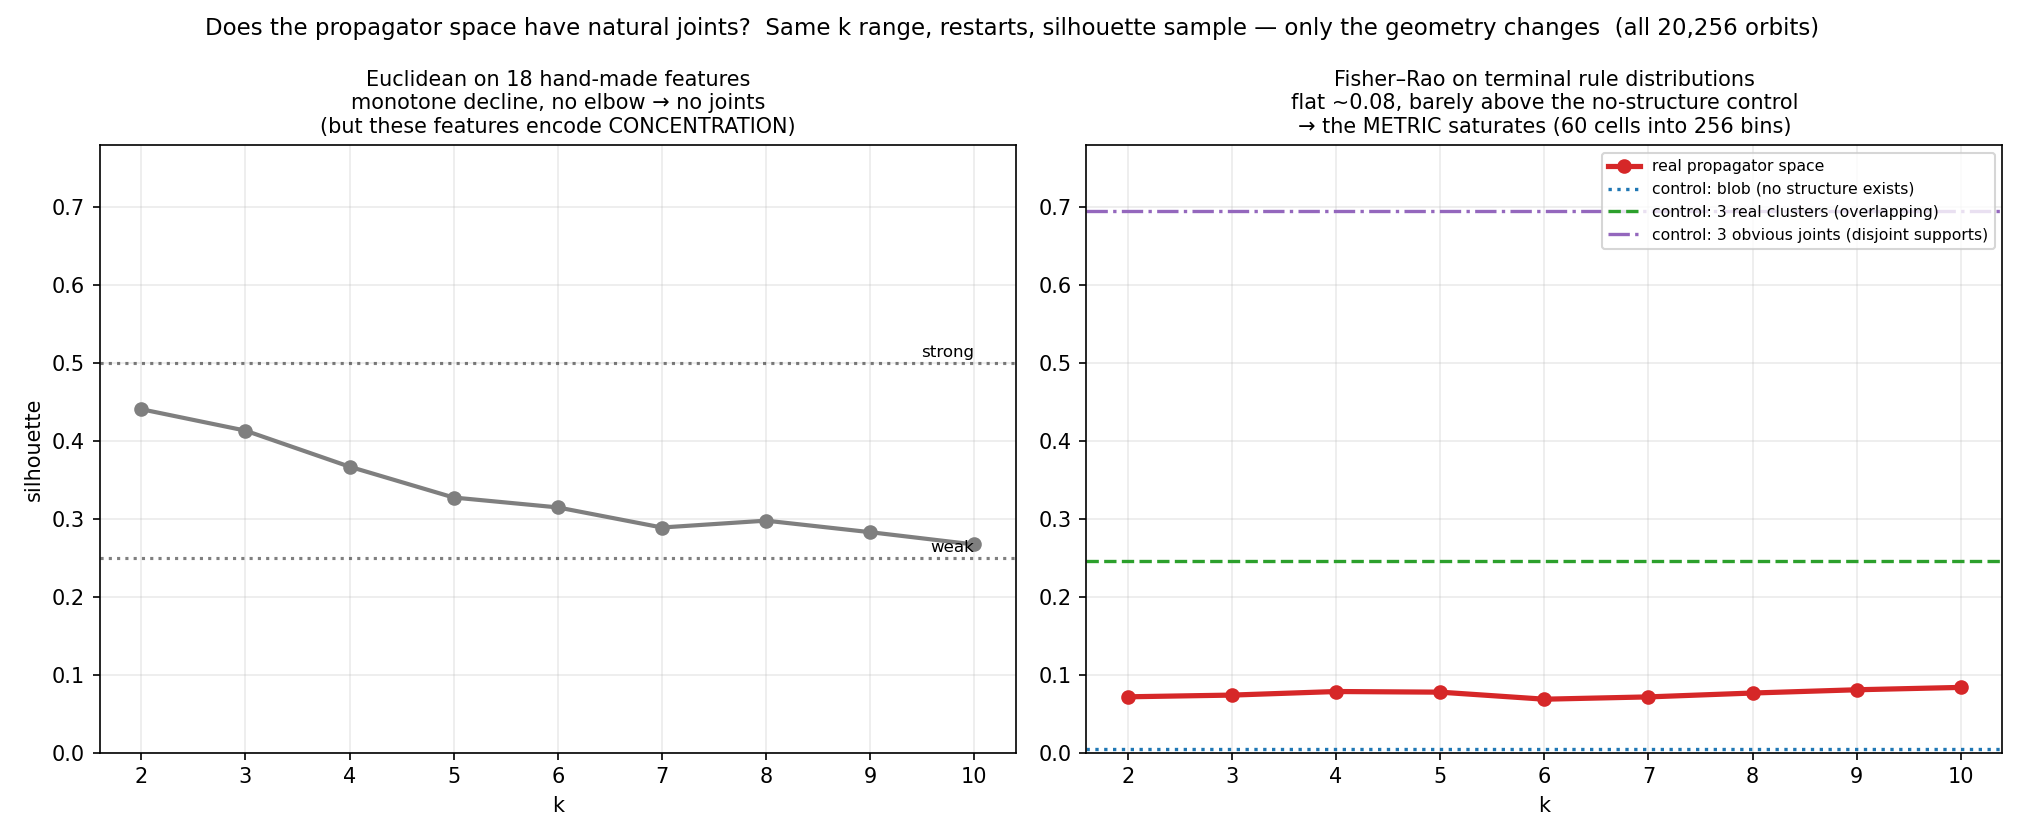
\includegraphics[width=\linewidth]{figures/fisher_rao_vs_euclidean.png}
  \caption{Fisher--Rao and Euclidean silhouettes over the census, with
  matched controls. The real data sits an order of magnitude below
  ``obvious joints'' and only slightly above a structureless blob.}
  \label{fig:fr}
\end{figure}

\subsection{Wasserstein-1 under a forced Hamming ground metric}

The ground metric here is \emph{forced, not chosen}, which is the reason to
trust it. The operator \texttt{rule-permute} writes exactly one bit, so a
propagator step \emph{is} a Hamming step and rule space \emph{is} the
8-bit cube. Moreover the \texttt{legacy}$\to$\texttt{standard} rule
renumbering is a bit \emph{permutation}, which preserves Hamming distance
--- so the ground metric is convention-independent. We are not choosing a
geometry and hoping; the dynamics chose it.

The peak silhouette is \textbf{0.176} (at $k=3$) against a $0.088$ blob and
$0.690$ for real structure (Figure~\ref{fig:w1}). Flat.

\begin{figure}[htbp]
  \centering
  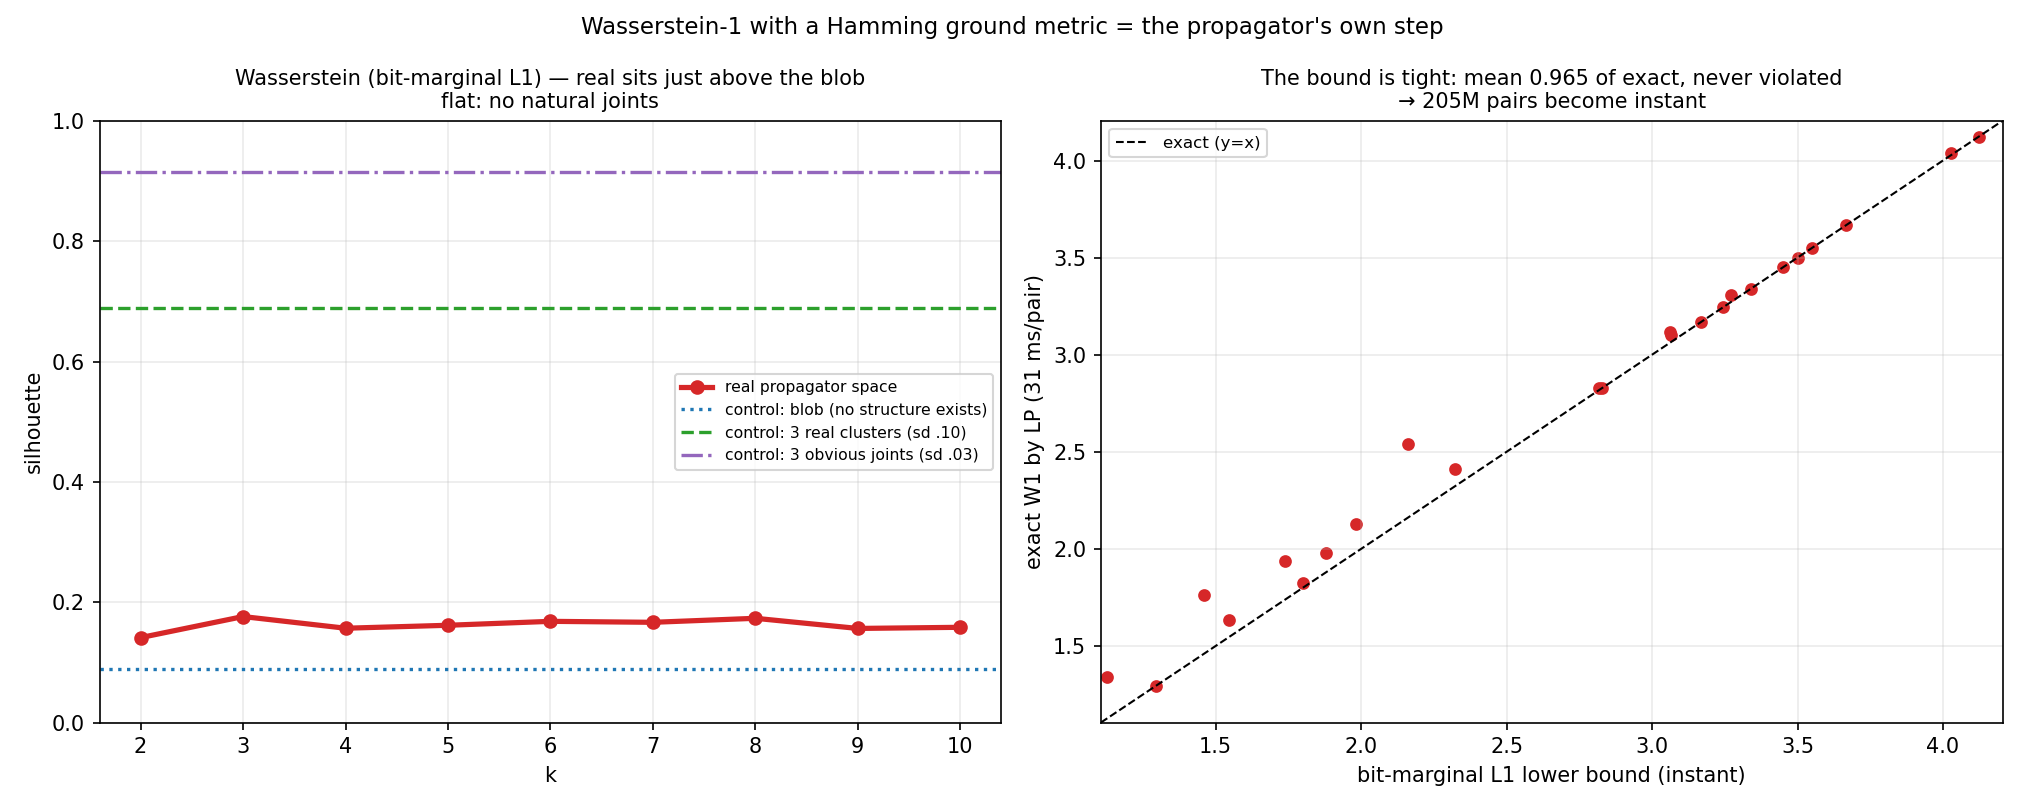
\includegraphics[width=\linewidth]{figures/wasserstein.png}
  \caption{Wasserstein-1 under the Hamming ground metric: mean-field bound
  tightness (left) and the flat silhouette against controls (right).}
  \label{fig:w1}
\end{figure}

\subsection{It survives its best attack}

The obvious objection is saturation: the terminal distributions occupy few
bins, so any distributional metric might be measuring sparsity rather than
structure. We tested it by pooling the last 20 generations, which gives
distributions roughly $20\times$ denser --- occupied bins rise from
\textbf{43.8 to 118.9} --- and measurably reduces saturation (mean pairwise
Fisher--Rao falls from \textbf{2.781 to 2.553}, computed exactly over all
$\binom{20256}{2} \approx 205\text{M}$ pairs). The silhouette
\textbf{stayed flat} ($0.084 \to 0.106$).

\dnote{The 2.781 $\to$ 2.553 pair is recomputed from
\texttt{data/propagator-metric/\{terminal,pooled-dists-K20\}.f64} for this
draft, exactly over the full population --- not sampled. Rows are
renormalised first: the stored rows are \emph{counts} summing to 180
(terminal: 60 cells $\times$ 3 seeds) and 3600 (pooled: $\times$ 20
generations), not probabilities. TN-propagator-paper.md reports
2.600 $\to$ 2.301 for the same quantity and \emph{no artefact reproduces
those figures} --- a 600-row sample gives 2.775 $\to$ 2.538, an
evenly-spaced 1000-row sample gives 2.787 $\to$ 2.560, and the exact
full-population value is 2.781 $\to$ 2.553. The \emph{direction and the
conclusion are unaffected} (saturation drops by a comparable margin;
silhouette stays flat), but the TN pair must be reconciled --- most likely
it came from a different row subset or an earlier normalisation. See
\texttt{README.md} in this directory.}

So the metric was saturating \emph{and} the space has no joints. Those are
two independent facts, and we had conflated them.

\subsection{An algebraic joint the metrics cannot see}
\label{sec:parity}

Every instrument above measures \emph{distance}. Each returns the same verdict:
no joints. We now report a partition of the same 20{,}256 orbits that is not a
distance at all, is computed from the operator alone with no simulation, and
predicts the census.

\subsubsection{The partition}

A propagator's shape map $\sigma$ is a permutation of the eight neighbourhoods.
Our Lean development proves
\texttt{bool\_fixed\_exists\_iff\_hasAlternatingColouring}: a Boolean fixed
point of $\sigma$ exists \emph{iff every cycle of $\sigma$ is even}. A fixed
point is a configuration the propagator cannot leave --- so an all-even $\sigma$
\emph{can} settle, and settling is death; an $\sigma$ with any odd cycle has no
fixed point to fall into.

The count is closed-form. Permutations of $2n$ with all cycles even number
$((2n-1)!!)^2$, so for $S_8$
\[
  \#\{\sigma : \text{all cycles even}\} = (7!!)^2 = 105^2 = 11{,}025
  \quad\text{of}\quad 8! = 40{,}320,
\]
i.e.\ $27.34\%$, with the remaining $29{,}295$ possessing an odd cycle. The
census, indexed by mirror orbits, contains $5{,}535$ all-even orbits of
$20{,}256$ --- $27.32\%$, matching the closed form. \emph{The composition of the
family is derivable without running anything.}

\subsubsection{It predicts the census}

\begin{table}[htbp]
  \centering
  \caption{Cycle parity against the full census (20{,}256 orbits, 3 seeds each).
  Parity is computed from $\sigma$; nothing in the simulation knows about it.}
  \label{tab:parity}
  \begin{tabular}{lrrrr}
    \toprule
    class & $n$ & died before horizon & mean death & mean terminal rules \\
    \midrule
    all-even (fixed point exists) & 5{,}535 & 1{,}445 ($26.1\%$) & 108.76 & 15.26 \\
    any-odd (no fixed point)      & 14{,}721 & 766 ($5.2\%$)     & 119.18 & 24.10 \\
    \bottomrule
  \end{tabular}
\end{table}

All-even orbits die \textbf{five times} as often and retain \textbf{a third
fewer} terminal rules. They are $27.3\%$ of the family and $65.4\%$ of the
deaths.

A prospective test, run after the prediction was registered and on operators not
previously built. \texttt{rot2} ($k \mapsto k+2$) has cycle type $(4,4)$ ---
all-even --- and collapses to a terminal diversity of $4$. \emph{Reduce} it, i.e.\
rotate a sub-orbit and hold the remaining registers fixed: every held register
becomes a $1$-cycle, $1$ is odd, the all-even condition breaks, and the fixed
point ceases to exist. The same rotation then sustains diversity $64$.

\begin{center}
\begin{tabular}{llr}
  \toprule
  $\sigma$ & cycle type & terminal diversity \\
  \midrule
  \texttt{rot2}, $k \mapsto k+2$        & $(4,4)$             & 4 \\
  \texttt{rot1}, $k \mapsto k+1$        & $(8)$               & 10--14 \\
  reduced \texttt{rot2} on $\{0,2,4,6\}$ & $(4,1,1,1,1)$       & 28--30 \\
  reduced \texttt{rot2} on $\{0,2,4\}$   & $(3,1,1,1,1,1)$     & 64--67 \\
  reduced \texttt{rot2} on $\{0,2\}$     & $(2,1,1,1,1,1,1)$   & 56--66 \\
  \bottomrule
\end{tabular}
\end{center}

Both all-even operators collapse; all three any-odd operators do not. The only
difference between the first and third rows is \emph{which registers are held}.

\subsubsection{What is and is not claimed}

Parity is \textbf{not} a clean partition of outcomes: $73.9\%$ of all-even
orbits survive to the horizon. This is expected --- the theorem gives
\emph{existence} of a fixed point, not \emph{attainment}. An all-even operator
can settle; whether it does depends on the initial condition. Parity is a strong
statistical joint, not a law about individual runs, and the $5.2\%$ of any-odd
orbits that die are unexplained by it.

The point stands nonetheless, and it revises this paper's own headline. The
family has \emph{no geometric structure and complete combinatorial structure at
the same time}, and these are not in tension. Cycle parity is not a metric
property: two permutations one transposition apart can fall on opposite sides,
so Euclidean, Fisher--Rao and Wasserstein-1 are constitutionally unable to see
it. Our fail bank is a fail bank of \emph{distances}. The joint was always
there, in the algebra, and it is four lines of Lean and a double factorial away.

\subsection{Conclusion}

A continuum with a slight non-uniformity, not a set of kinds
(Figure~\ref{fig:contact}).

\begin{figure}[htbp]
  \centering
  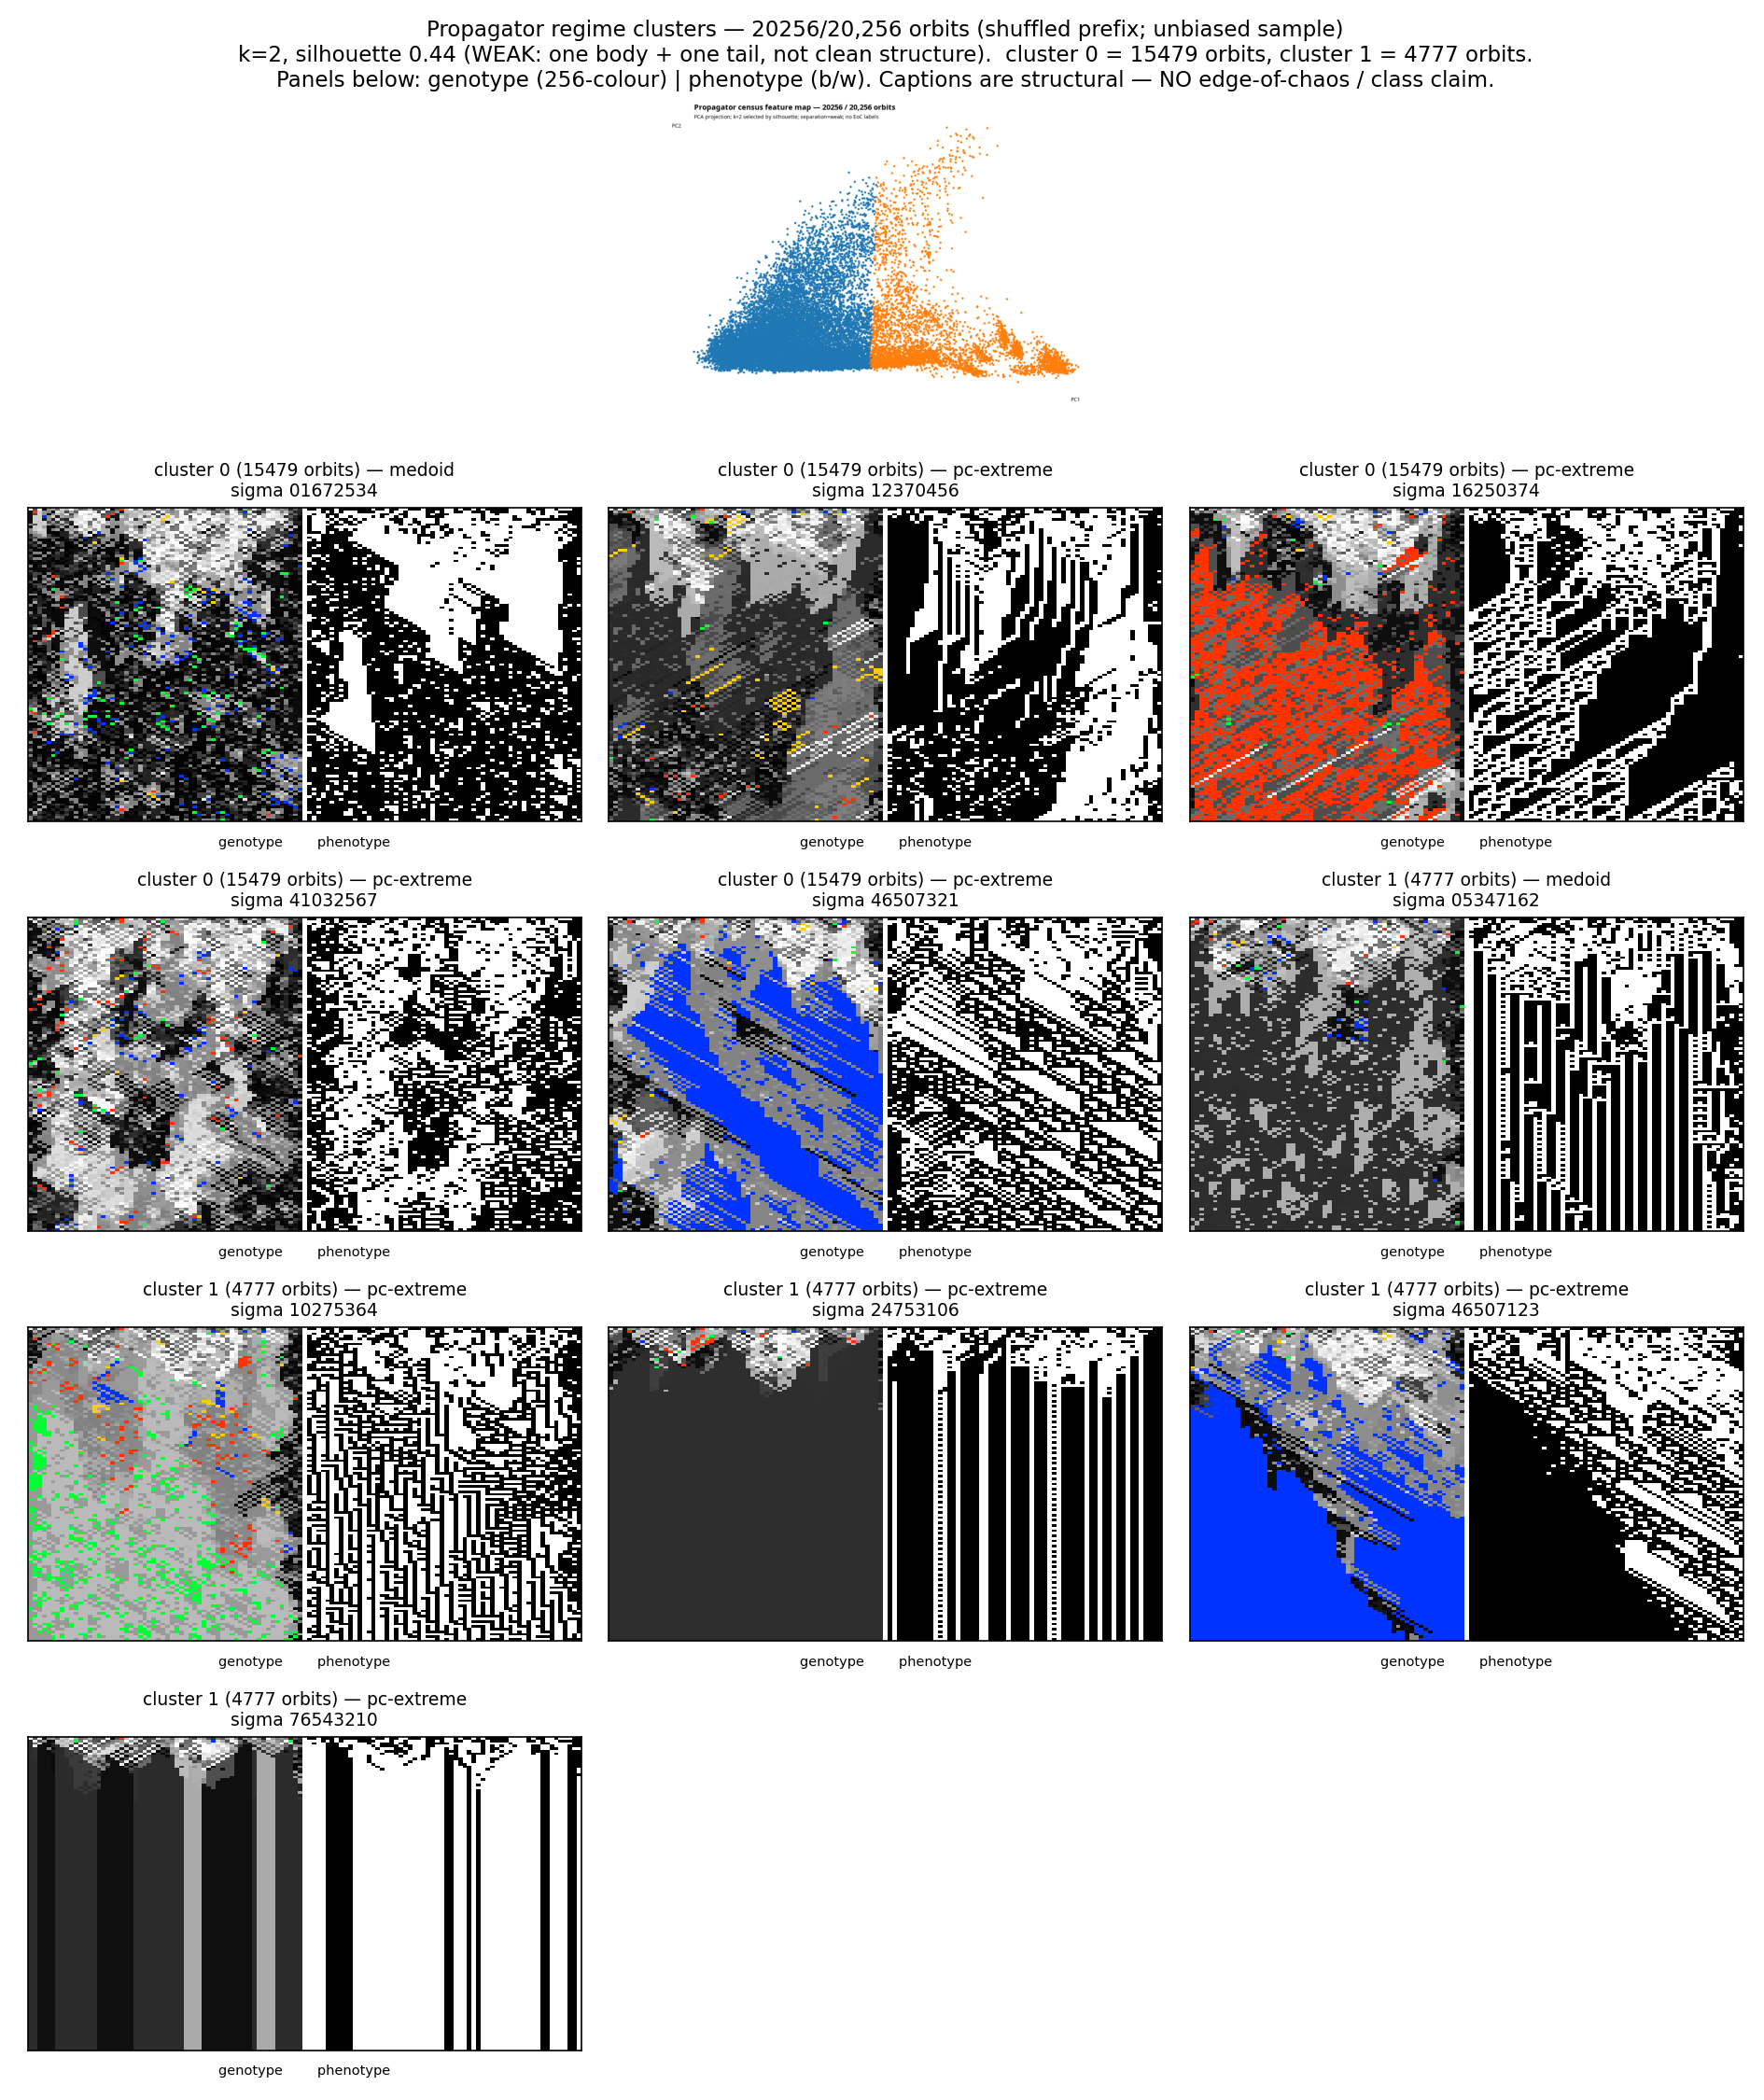
\includegraphics[width=0.85\linewidth]{figures/contact_sheet.png}
  \caption{Ten exemplars spanning the census, genotype and phenotype, full
  coverage --- not a curated selection. The eye finds these obviously
  different; no metric we ran does.}
  \label{fig:contact}
\end{figure}

% =====================================================================
\section{Methods That Survived}
\label{sec:methods}
% =====================================================================

\subsection{The mean-field embedding}

Hamming distance is a sum over bits, so $W_1$ nearly decomposes into
per-bit marginal differences. This yields a certified lower bound
\[
  W_1(p,q) \;\ge\; \sum_{b=0}^{7} \bigl| \mathbb{E}_p[b] - \mathbb{E}_q[b] \bigr|,
\]
measured at a mean of \textbf{0.965 of exact} over sampled pairs (never
violated; minimum 0.830).

The eight numbers are not merely a compression. They are interpretable ---
the per-neighbourhood mean response of the rule population --- dense, and
exactly the object the propagator acts on. And they make the census
tractable: \textbf{205M pairs become instant}.

We tried Sinkhorn \parencite{cuturi2013sinkhorn} and dropped it: at 43\,ms
per pair it was \emph{slower} than the exact LP at 31\,ms, the entropic
regularisation buying nothing at this problem size.

\dnote{The TN reports bound tightness as ``0.957--0.965 of exact''. The
artefact (\texttt{wasserstein.json}) records
\texttt{tightness\_mean}~$=0.9647$ and \texttt{tightness\_min}~$=0.8297$
over 24 pairs. The draft uses the artefact. The TN's lower figure of 0.957
does not appear in the artefact and may be a mean from an earlier run ---
reconcile.}

\subsection{Ollivier--Ricci curvature as navigation}

A space with no clusters offers nothing to hop between, so we asked for a
local direction instead. Ollivier--Ricci curvature
\parencite{ollivier2009ricci} on the census graph gives mean
$\kappa = +0.085$ with \textbf{30.3\% of edges negative}
(Figure~\ref{fig:curv}). The negatively-curved edges are the frontier ---
the ``propose here'' signal for a search that cannot navigate by cluster
membership.

The structural finding: \textbf{80\% of the most negatively-curved edges
connect $\sig$ differing by a single transposition}. A minimal edit to
$\sig$ sits at a branch point. This survives its artifact test --- the
statistic holds at 83\% with near-duplicates excluded, where $1/d$
amplification could otherwise have manufactured it.

\begin{figure}[htbp]
  \centering
  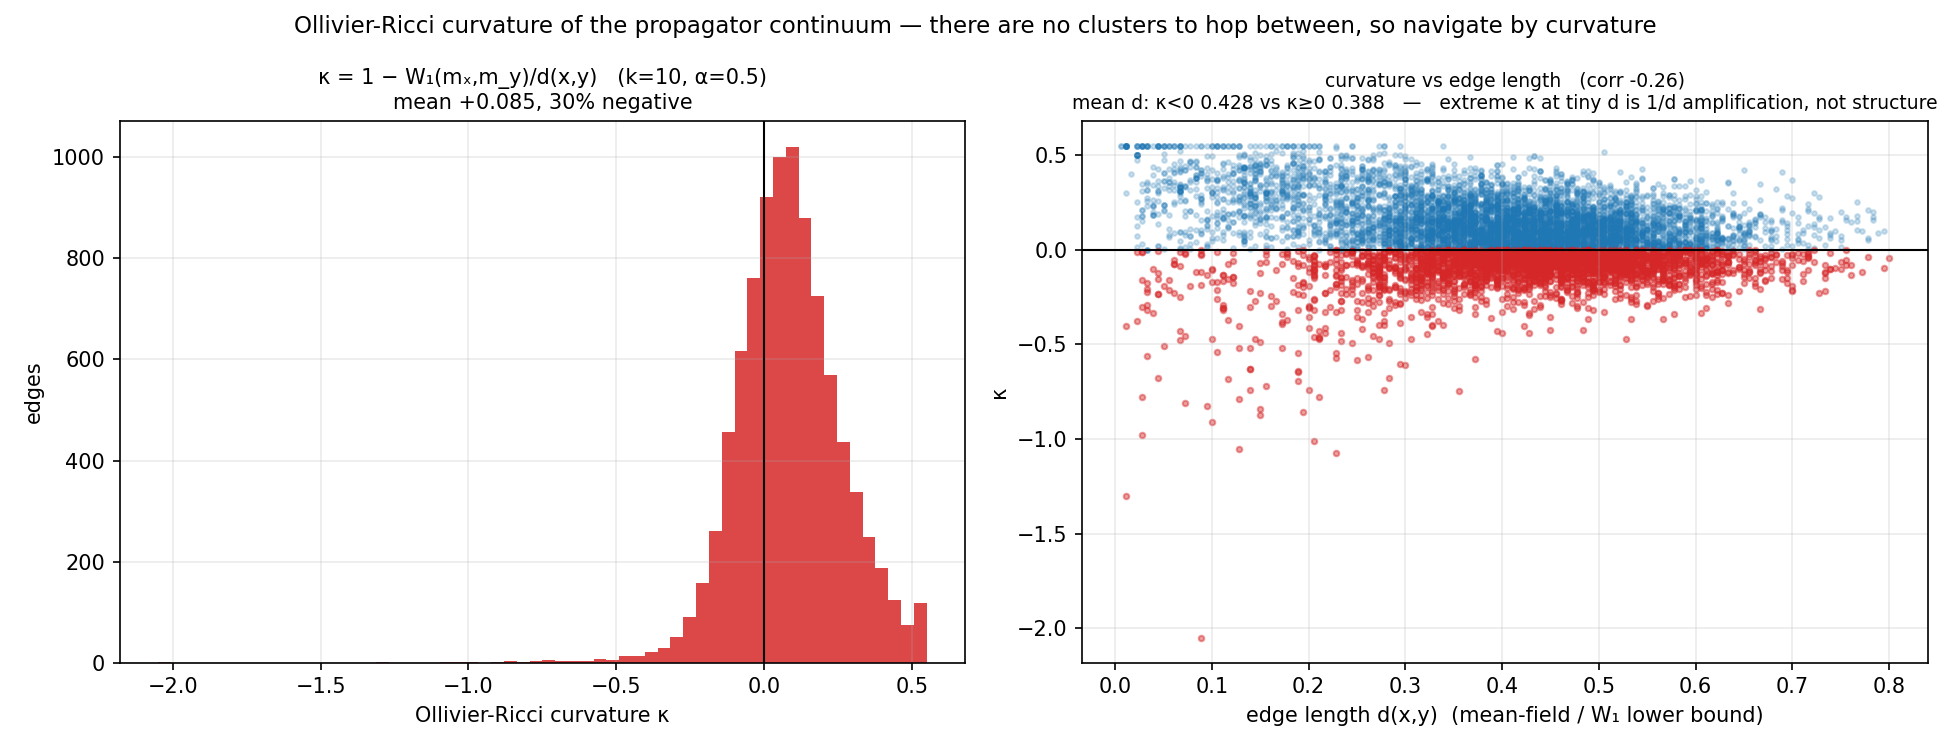
\includegraphics[width=\linewidth]{figures/curvature.png}
  \caption{Ollivier--Ricci curvature over the census graph
  ($k=10$, $\alpha=0.5$, 2000 nodes, 9157 edges).}
  \label{fig:curv}
\end{figure}

% =====================================================================
\section{Reproducibility}
\label{sec:repro}
% =====================================================================

\dnote{TN says: ``a genuine strength --- lead with it''. It is currently
Section~8, which is not leading with it. Options: promote to the
Introduction as a contribution bullet (partly done), or open the paper with
the reconstruction-as-method framing. Resolve when the intro is rewritten.}

Every claim in Sections~\ref{sec:propagator}--\ref{sec:methods} is backed
by a fingerprinted artefact.

\begin{itemize}
  \item \textbf{Fingerprinting.} The census fingerprint
  \texttt{ac2ff1681eae5b85} covers the SHA-256 of every source input: the
  driver, the lexical-binding Elisp worker, the orbit witness, the harness,
  the protocol, and every vendored MetaCA file. Each compressed census
  carries an atomic manifest with its own SHA-256; resume rejects absent,
  stale, or checksum-mismatched files.

  \item \textbf{Any prefix is a uniform sample.} The build order is a
  seeded shuffle, so a partial census is an unbiased sample of the full
  one. This is not a claim --- it is measured: the 580-orbit overnight
  preview (2.86\% coverage) predicted the full 20{,}256-orbit result to
  0.7\%.

  \item \textbf{Byte-identical determinism} verified by deleting a seed's
  artefact and regenerating it.

  \item \textbf{The original code is evidence, not a dependency.}
  \texttt{vendor/metaca/} carries the 2014 and 2015 Emacs Lisp unedited.
  The reconstruction loads it through a side-file wrapper and never
  modifies it; write positions are observed after Emacs clamps, so the
  histograms measure behaviour rather than inferring it from source.
\end{itemize}

% =====================================================================
\section{Discussion}
% =====================================================================

\owed{Not written. Sketch of what belongs here:
(i) what the propagator family \emph{is} good for, if not for
edge-of-chaos measurement --- the curvature result suggests it is a search
space with a usable local signal;
(ii) the reconstruction-as-method argument: a twelve-year-old bug was
recoverable, correctable, and generative, which says something about
keeping code as evidence;
(iii) the honest limits (three seeds, width 60, no blob control on the
Euclidean sweep);
(iv) what would change our mind --- what a real edge-of-chaos instrument
would have to look like given Culik \& Yu, and why we think the answer is
``it would have to be a construction, like Cook's, not a statistic''.}

\subsection{What is deliberately not claimed}

\dnote{Keep this subsection. It is what makes the rest credible, and the TN
is explicit that both items below are \emph{out}.}

\paragraph{The transfer thesis is not established.}
An earlier framing of this work reached for ``patterns of improvisation'' ---
computational intelligence that transfers domain to domain. We do not claim
it. The tokamak controller is parked with an unanchored objective, and
while the ant C-vector authority gate passes, the xeno loop is
undemonstrated. Gesturing at transfer would be the exciting version of this
paper that the evidence does not support.

\paragraph{The tokamak numbers are not banked.}
Greedy scores 0.2458 against a best-fixed 0.2418 on 3 of 4 seeds --- with
one seed losing by more than the mean effect size. Suggestive; not a
result.

\owed{Decide whether the tokamak appears at all. If it does not,
\texttt{figures/tokamak\_run\_figure.png} is unused and the two paragraphs
above shrink to one sentence. The TN lists the figure as
``if the tokamak appears at all''. Current recommendation: cut it --- the
paper is complete without it and the numbers invite a fight we do not need
to have.}

% =====================================================================
\printbibliography

\end{document}
